\documentclass{article}
\usepackage{graphicx} % Required for inserting images
\usepackage{subcaption}
\usepackage{cancel}
\usepackage[margin=0.65in]{geometry}
\usepackage{enumitem}
\usepackage{graphicx}
\usepackage{float}
\usepackage{amsmath} % Required for \text{} and align environment
\usepackage{tikz}
\usetikzlibrary{shapes,arrows,positioning}
\usepackage{tcolorbox} % Required for colored answer boxes
\usepackage{multicol}
\definecolor{lightyellow}{rgb}{1, 1, 0.8}

\setlist{itemsep=1pt, parsep=5pt, topsep=5pt}
\setlength{\parindent}{0pt}
\setcounter{secnumdepth}{0}


\title{Computer Architecture Phase 1} 
\author{Demian Marín Martínez - dm6430}
\date{Friday 7 November 2025}


\begin{document}

\maketitle

\begin{enumerate}                                                                                                                                                                                                                                       
  \item Draw the schematic for a single stage processor and fill in your code in the to run the simulator. (20 points)                                                                                                                                  
  \item Draw the schematic for a five stage pipelined processor and fill in your code to run the simulator. The processor should be able to take care of RAW and control hazards by stalling and forwarding. (20 points)                                
  \item Measure and report average CPI, Total execution cycles, and Instructions per cycle for both these cores by adding performance monitors to your code. (Submit code and print results to console or a file.) (5 points)                           
  \item Compare the results from both the single stage and the five stage pipelined processor implementations and explain why one is better than the other. (5 points)                                                                                  
  \item What optimizations or features can be added to improve performance? (Extra credit 1 point) 
\end{enumerate}

1.
% Single Stage Processor Diagram
%
% This diagram shows the basic components of a single-stage RISC-V processor.
%
% Components:
% - PC (Program Counter): Holds the address of the instruction being fetched.
%   - Input: Next instruction address.
%   - Output: Current instruction address.
% - Instruction Memory: Stores the program instructions.
%   - Input: Instruction address from PC.
%   - Output: The instruction itself.
% - Register File: Holds the processor's general-purpose registers.
%   - Input: Register numbers to read, data to write, write enable signal.
%   - Output: Data from specified registers.
% - ALU (Arithmetic Logic Unit): Performs calculations.
%   - Input: Operands from the register file or immediate values.
%   - Output: The result of the operation.
% - Data Memory: Stores the program's data.
%   - Input: Address from ALU, data to write.
%   - Output: Data read from memory.
% - MUX (Multiplexer): Selects one of several inputs.
%   - PC MUX: Selects the next PC value (either PC+4 or a branch target).
%   - WB MUX: Selects the data to be written back to the register file (either ALU result or memory data).
% - +4: An adder to calculate the address of the next instruction in sequence.

\begin{figure}[H]
    \centering
    \resizebox{\textwidth}{!}{
    \begin{tikzpicture}[node distance=2.5cm, auto, >=stealth']
        % Nodes
        \node (pc) [draw, rectangle] {PC};
        \node (instr_mem) [draw, rectangle, right=of pc] {Instruction Memory};
        \node (reg_file) [draw, rectangle, right=of instr_mem] {Register File};
        \node (alu) [draw, rectangle, right=of reg_file] {ALU};
        \node (data_mem) [draw, rectangle, right=of alu] {Data Memory};
        \node (wb_mux) [draw, rectangle, right=of data_mem] {MUX};
        \node (add4) [draw, circle, below=of pc] {+4};
        \node (mux_pc) [draw, rectangle, left=of pc] {MUX};

        % Main data path
        \draw[->] (pc.east) -- (instr_mem.west);
        \draw[->] (instr_mem.east) -- (reg_file.west);
        \draw[->] (reg_file.east) -- (alu.west);
        \draw[->] (alu.east) -- (data_mem.west);
        \draw[->] (data_mem.east) -- (wb_mux.west);

        % Write-back path from ALU
        \draw[->] (alu.south) |- ++(0,-1.5) -| (wb_mux.south);

        % Write-back to register file
        \draw[->] (wb_mux.north) |- ++(0,1) -| (reg_file.east);

        % PC update logic
        \draw[->] (pc.south) -- (add4.north);
        \draw[->] (add4.west) -| (mux_pc.south);
        \draw[->] (mux_pc.east) -- (pc.west);
        
        % Branch logic from ALU to PC MUX
        \draw[->] (alu.south) |- ++(0,-2) -| (mux_pc);
    \end{tikzpicture}
    }
    \caption{Single Stage Processor}
    \label{fig:single_stage}
\end{figure}

2.
% Five-Stage Pipelined Processor Diagram
%
% This diagram shows a five-stage pipelined RISC-V processor.
% Pipelining increases throughput by overlapping the execution of multiple instructions.
%
% Stages:
% - IF (Instruction Fetch): Fetches the instruction from memory.
% - ID (Instruction Decode): Decodes the instruction and reads from the register file.
% - EX (Execute): Performs the ALU operation.
% - MEM (Memory Access): Reads from or writes to data memory.
% - WB (Write-Back): Writes the result back to the register file.
%
% Pipeline Registers (IF/ID, ID/EX, EX/MEM, MEM/WB):
% - These registers are placed between stages to hold the intermediate results and control signals for the instruction being processed in that stage.
%
% Hazard Unit:
% - Detects data and control hazards. It can stall the pipeline or control the forwarding paths to resolve these hazards.
%
% Forwarding Paths:
% - These paths (dashed lines) allow the result of an instruction in a later stage (EX or MEM) to be used as an operand for an instruction in an earlier stage (ID/EX), avoiding unnecessary stalls.

\begin{figure}[H]
    \centering
    \resizebox{\textwidth}{!}{
    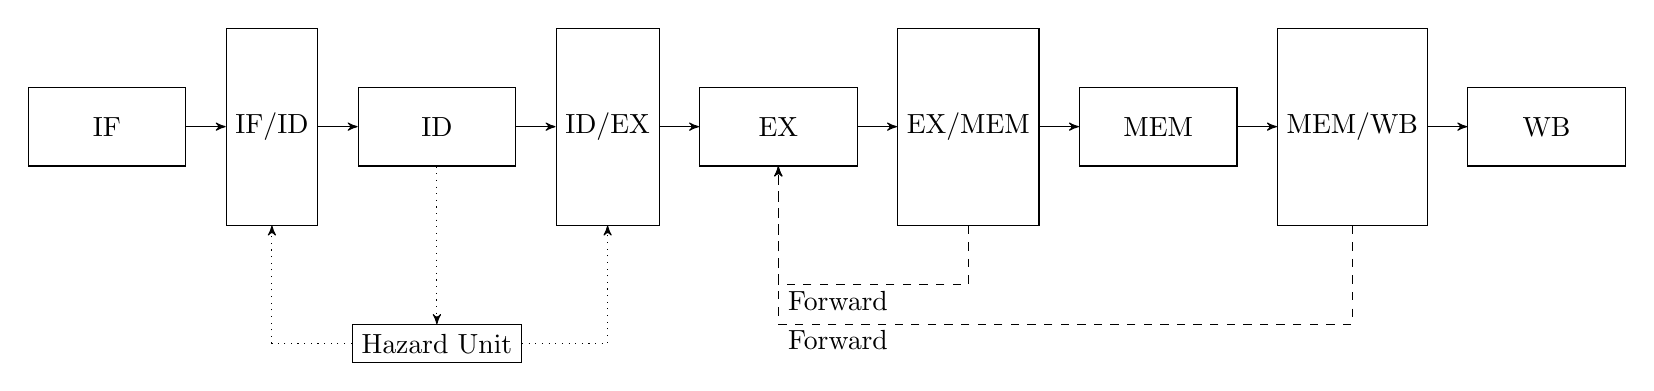
\begin{tikzpicture}[
        node distance=1cm,
        auto,
        >=stealth',
        block/.style={draw, rectangle, minimum width=2cm, minimum height=1cm},
        pipeline/.style={draw, rectangle, minimum height=2.5cm}
    ]
        % Nodes
        \node (if) [block] {IF};
        \node (if_id) [pipeline, right=0.5cm of if] {IF/ID};
        \node (id) [block, right=0.5cm of if_id] {ID};
        \node (id_ex) [pipeline, right=0.5cm of id] {ID/EX};
        \node (ex) [block, right=0.5cm of id_ex] {EX};
        \node (ex_mem) [pipeline, right=0.5cm of ex] {EX/MEM};
        \node (mem) [block, right=0.5cm of ex_mem] {MEM};
        \node (mem_wb) [pipeline, right=0.5cm of mem] {MEM/WB};
        \node (wb) [block, right=0.5cm of mem_wb] {WB};

        % Connections
        \draw[->] (if) -- (if_id);
        \draw[->] (if_id) -- (id);
        \draw[->] (id) -- (id_ex);
        \draw[->] (id_ex) -- (ex);
        \draw[->] (ex) -- (ex_mem);
        \draw[->] (ex_mem) -- (mem);
        \draw[->] (mem) -- (mem_wb);
        \draw[->] (mem_wb) -- (wb);

        % Hazard Unit
        \node (hazard) [draw, rectangle, below=2cm of id] {Hazard Unit};
        \draw[->, dotted] (id.south) -- (hazard);
        \draw[->, dotted] (hazard.west) -| (if_id.south);
        \draw[->, dotted] (hazard.east) -| (id_ex.south);

        % Forwarding paths
        \draw[->, dashed] (ex_mem.south) -- ++(0,-0.75) -| (ex.south) node[midway, right, yshift=-0.2cm] {Forward};
        \draw[->, dashed] (mem_wb.south) -- ++(0,-1.25) -| (ex.south) node[midway, right, yshift=-0.2cm] {Forward};

    \end{tikzpicture}
    }
    \caption{Five Stage Pipelined Processor}
    \label{fig:five_stage}
\end{figure}

3.
The performance metrics for the single-stage and five-stage processors are as follows:

\begin{itemize}
    \item \textbf{Single Stage Core}
    \begin{itemize}
        \item Number of cycles taken: 36
        \item Cycles per instruction (CPI): 1.0286
        \item Instructions per cycle (IPC): 0.9722
    \end{itemize}
    \item \textbf{Five Stage Core}
    \begin{itemize}
        \item Number of cycles taken: 9
        \item Cycles per instruction (CPI): 1.5
        \item Instructions per cycle (IPC): 0.6667
    \end{itemize}
\end{itemize}

4.
The five-stage pipelined processor is better than the single-stage processor, even though its CPI is higher. Here's why:

\begin{itemize}
    \item \textbf{Throughput:} The five-stage processor has a much higher throughput. It can execute multiple instructions concurrently in different stages of the pipeline. This is evident from the total execution cycles: the five-stage processor took only 9 cycles to complete the program, while the single-stage processor took 36 cycles.
    \item \textbf{Clock Speed:} Pipelining allows for a faster clock speed. In a single-stage processor, the clock cycle is determined by the longest instruction. In a pipelined processor, the clock cycle is determined by the longest stage, which is much shorter. This means that even though an instruction takes 5 cycles to complete, a new instruction can start every cycle, leading to a significant speedup.
    \item \textbf{CPI vs. IPC:} While the single-stage processor has a better CPI (closer to 1), this is misleading. The CPI for the pipelined processor is higher due to stalls from hazards (data and control). However, because the clock cycle is much faster and it has higher throughput, the overall performance is better. The IPC for the single-stage processor is higher because it completes an instruction in almost every cycle, but each of those cycles is much longer.
\end{itemize}

In conclusion, the five-stage pipelined processor is significantly better due to its ability to overlap the execution of instructions, leading to a much lower total execution time.

5.
Several optimizations and features can be added to improve the performance of the five-stage pipelined processor:

\begin{itemize}
    \item \textbf{Branch Prediction:} To reduce the penalty of control hazards, a branch predictor can be implemented. Instead of stalling the pipeline every time a branch is encountered, the processor can predict the outcome of the branch and speculatively fetch and execute instructions from the predicted path. If the prediction is correct, there is no penalty. If it is incorrect, the pipeline is flushed, but this is often better than always stalling.
    \item \textbf{Superscalar Execution:} A superscalar processor can execute more than one instruction per clock cycle by having multiple pipelines. For example, a 2-way superscalar processor could fetch, decode, and execute two instructions at a time, potentially doubling the IPC.
    \item \textbf{Out-of-Order Execution:} This allows the processor to execute instructions as soon as their operands are available, rather than strictly in program order. This can hide the latency of instructions with long execution times (like loads from memory) and improve the utilization of the execution units.
    \item \textbf{More Advanced Forwarding:} While the current implementation has forwarding, more complex forwarding paths can be added to handle more types of data hazards without stalling.
    \item \textbf{Cache Hierarchy:} Adding a multi-level cache (L1, L2, L3) can significantly reduce the average memory access time. A faster cache can provide data to the processor much more quickly than main memory, reducing the number of stalls due to memory access.
\end{itemize}


\end{document}
